\documentclass[bluish,slideColor,colorBG,pdf]{prosper}
\hypersetup{pdfpagemode=FullScreen}
\usepackage{graphicx,amsfonts,amsmath}
\usepackage{bm}
\def\baselinestretch{1.0}
\setlength{\topmargin}{-60pt}
\setlength{\textheight}{460pt}
\setlength{\oddsidemargin}{0pt}
\setlength{\evensidemargin}{0pt}
\setlength{\textwidth}{660pt}
\setlength{\footskip}{0pt}
\parindent 0.3in
\hyphenpenalty=10000
\tolerance=10000
\pagestyle{empty}

\def\Prob{{\rm Prob\;}}
\def\prob{{\rm \;Prob\;}}
\def\Var{{\rm Var}}        % Var
\def\Cov{{\rm Cov}}        % Cov

\DeclareSymbolFont{AMSb}{U}{msb}{m}{n}
\DeclareMathSymbol{\expect}{\mathalpha}{AMSb}{'105}

% bold math (use \bm{...})
\def\bm#1{\mathpalette\bmstyle{#1}}
\def\bmstyle#1#2{\mbox{\boldmath$#1#2$}}

\title{Week 9: Quantitative characters, comparative method, coalescents}
\author{Genome 570}
\institution{March, 2016}

\begin{document}

\maketitle

\begin{slide}[Replace]{ ``Pruning'' a tree in the Brownian motion case}

\centerline{\includegraphics[height=2.2in]{fig23-3.ydraw}}

\end{slide}

\begin{slide}[Replace]{What about quantitative characters? }
\bigskip

In the classical (Fisher, 1918) model of quantitative genetics, a quantitative character is a sum of contributions from different
loci, plus an independent environmental effect:
\bigskip

\[
\hspace*{0in}\hspace{-0.27in}P \ = \ \mu
 \ + \ \left\{
\begin{array}{c c}
{\rm AA} &  1.2 \\
{\rm Aa} &  0.8 \\
{\rm aa} &  0.7 
\end{array}
\right\} \ + \ 
\left\{
\begin{array}{c c}
{\rm BB} &  -0.02\\
{\rm Bb} &  0.00 \\
{\rm bb} &  0.01 
\end{array}
\right\} \ + \ 
\dots \ + \ 
\left\{
\begin{array}{c c}
{\rm ZZ} &  0.21 \\
{\rm Zz} &  0.21\\
{\rm zz} &  -0.17
\end{array}
\right\}
\ + \ \varepsilon
\]

In that case if locus is independently changing by (approximate) Brownian
motion, the character's phenotype will also change by approximate
Brownian motion.

\end{slide}

\begin{slide}[Replace]{What about quantitative characters? }
\bigskip

For neutral mutation and genetic drift, can show that for a quantitative
character with additive genetic variance $~\mathsf{V_A}~$ and population size $\mathsf{~N~}$
the variance through time of the genetic (additive) value of the population mean is:
\[
\mathsf{\Var (\Delta \bar{g}) \ = \ V_A / N}
\]
\noindent
so it is smaller the bigger the population is, as there is less genetic drift.

If mutation and drift are at equilibrium:
\[
\mathsf{\expect\left[V_A^{(t+1)}\right] \ = \ V_A^{(t)} \left(1 - \frac{1}{2N}\right) + V_M}
\]
\noindent
which lets us calculate what the additive genetic variance becomes, on
average.  This leads to a surprise ...

\end{slide}

\begin{slide}[Replace]{In neutral traits multational variance rules}
\bigskip

so that
\[
\mathsf{\expect\left[V_A\right] \ = \ 2N V_M}
\]

whereby
\[
\mathsf{\Var[\Delta {\bar g}] \ = \ \left(2N V_M \right) / N  \ = \  2 V_M},
\]
an analogue of Kimura's result for neutral mutation.
\medskip

\end{slide}

\begin{slide}[Replace]{Long-term change would mirror genetic variation}
\bigskip

There is a precise analogue of those equations for multiple characters, using matrices
instead of scalars in the equations.
\bigskip

Thus to transform characters to independent Brownian motions of equal
evolutionary variance, we could use their current additive genetic covariances
$\mathsf{{\bm V}_A}$,

\centerline{\includegraphics[width=2.5in]{neutralvar.idraw}}

We come up with new axes that vary independently among species.

The independent Brownian Motion on these axes shows that neutral variation
changes in the directions of the Principal Components of the original additive
genetic covariance matrix.

\end{slide}

\begin{slide}[Replace]{With selection ... life is harder}
\bigskip


There is the quantitative genetics formula of Wright and Fisher (1920's)
\[
\mathsf{\Delta z\ =\ h^2 S}
\]

and Russ Lande's (1976) recasting of that in terms of slopes of mean fitness
surfaces:
\[
\mathsf{S \ =\ V_P \; \frac{d \log\left({\bar w} \right)}{dx}}
\]

\[
\mathsf{\Delta z\  =\  (V_A/V_P)\; V_P\; \frac{d \log\left({\bar w} \right)}{dx}
= \ V_A\;\frac{d \log\left({\bar w} \right)}{dx}}
\]
\end{slide}

\begin{slide}[Replace]{Selection towards an optimum}
\bigskip

\centerline{\includegraphics[width=1.5in]{fig24-1.ydraw}}

If fitness as a function of phenotype is:
\[
\mathsf{w(x)\  = \ \exp\left[-\frac{(x-p)^2}{2 V_s} \right]},
\]
\noindent
Then the change of mean phenotype ``chases'' the optimum:
\[
\mathsf{m' - m\  =\  \frac{V_A}{V_s + V_P}\; (p - m)},
\]
\noindent
in each generation moving a constant fraction of the way to the optimum.

\end{slide}

\begin{slide}[Replace]{Genetic drift, mutation and selection give an OU
process}

\centerline{(The plots are from the same sets of random numbers)}
\begin{center}
\begin{tabular}{c c}
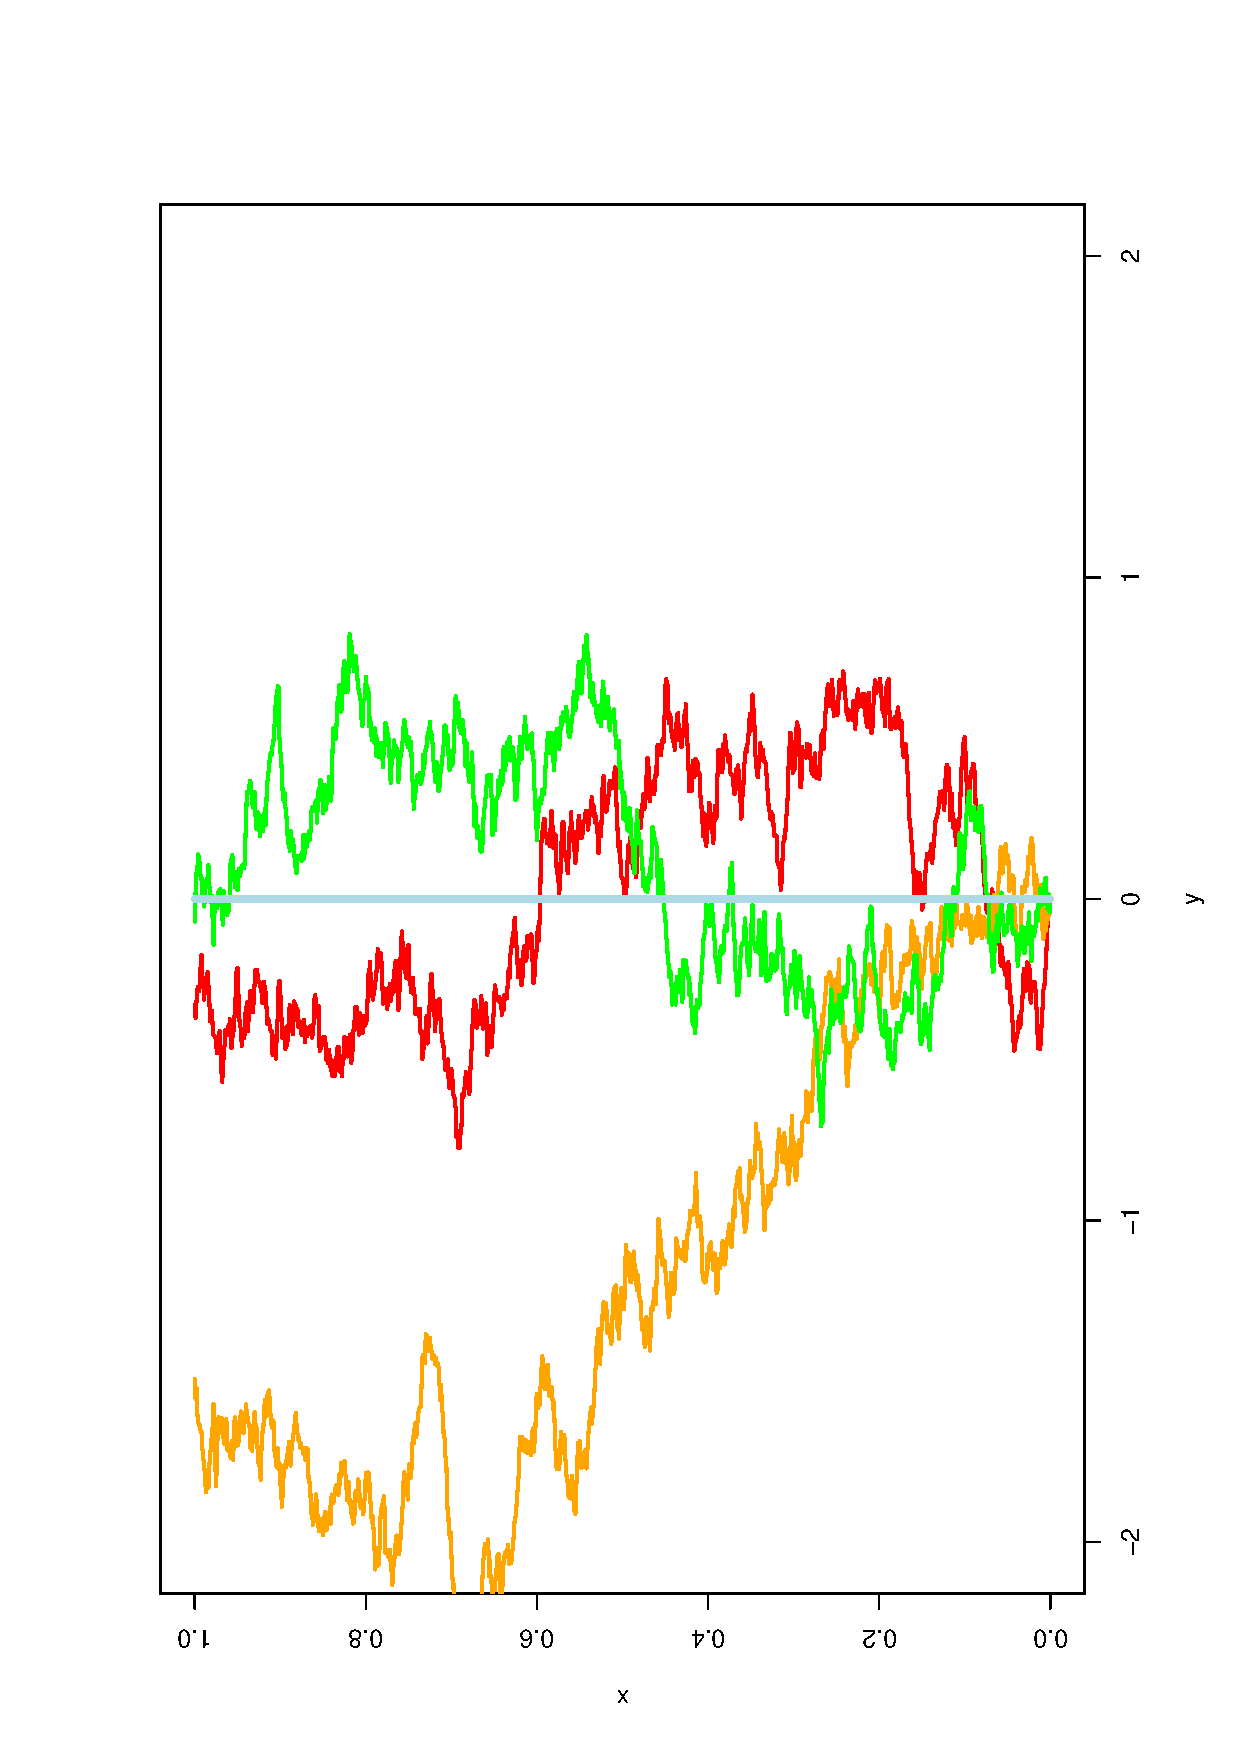
\includegraphics[width=2.0in]{bmplot.idraw} &
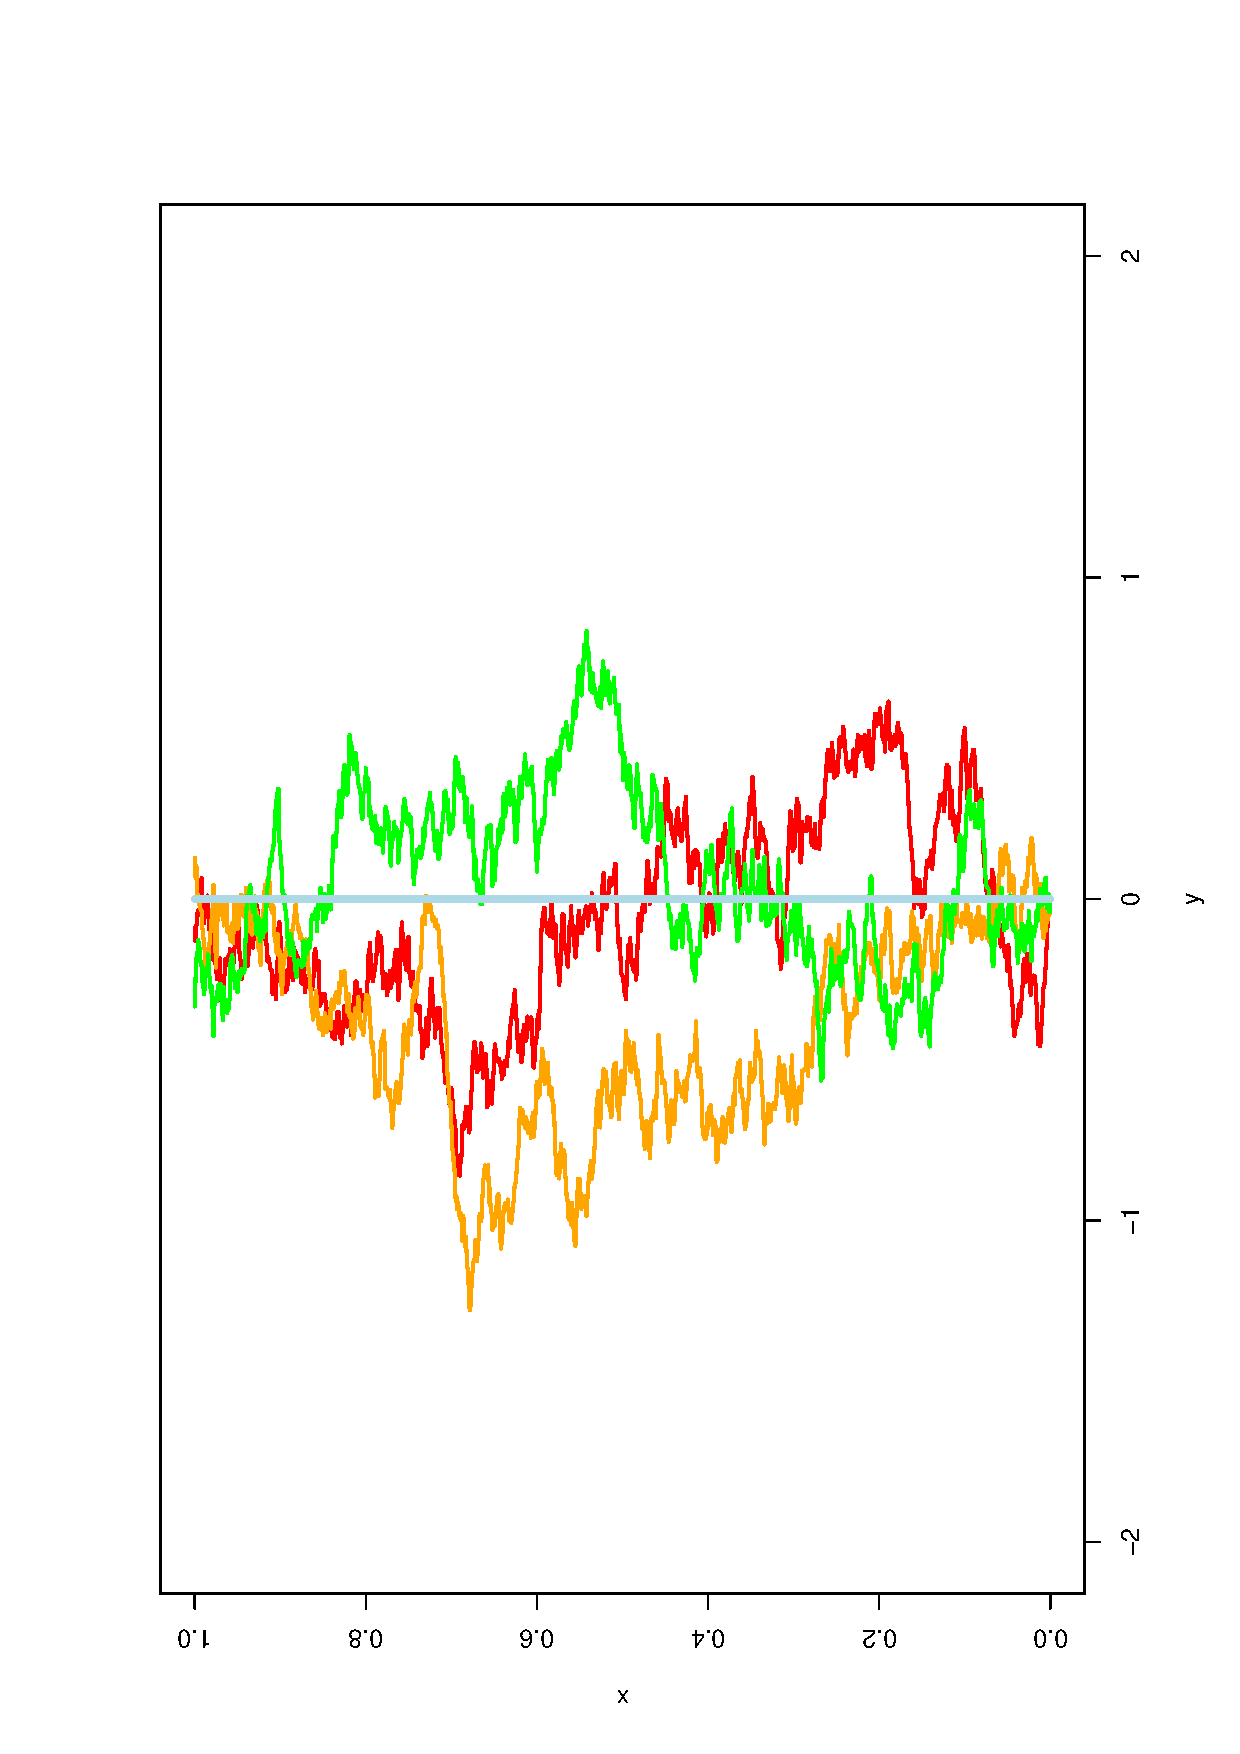
\includegraphics[width=2.0in]{ouplot.idraw} \\
Brownian motion & an OU process
\end{tabular}
\end{center}
\medskip

The process is approximately an Ornstein-Uhlenbeck Process, a relative of
Brownian Motion in which the particle is ``elastically bound'' (tethered
to a post by an elastic band).  
\bigskip

In this case the OU process has the particle wandering by genetic drift, but
constantly pulled toward the optimum value by natural selection.

\end{slide}

\begin{slide}[Replace]{A character changing by ``chasing'' an adaptive peak}
\bigskip

\centerline{\includegraphics[width=2in]{peakshift.ydraw}}
\bigskip

The course of change of the population mean is expected to be somewhat
smoother than the changes of the peak of the fitness surface.

\end{slide}

\begin{slide}[Replace]{Sources of evolutionary correlation among characters}
\bigskip

Variation (and covariation) in change of characters occurs for two reasons:
\medskip

\begin{enumerate}
\item Genetic drift, with the covariances being proportional to the additive genetic covariances
\item Selection, with the covariances being affected by both the additive genetic covariances and the covariation of the selection pressures.
\end{enumerate}

\end{slide}

\begin{slide}[Replace]{A simple example of selective covariance}
\bigskip

\noindent
\centerline{\includegraphics[width=4.7in]{selectcov.ydraw}}

\end{slide}

\begin{slide}[Replace]{A simulated example with two characters}
\bigskip

\centerline{After 100 generations:}
\medskip

\centerline{\includegraphics[width=2in]{fig4.100.idraw}}
\bigskip

Genetic covariances are negative, but the wanderings of the adaptive peak
in the two characters are positively correlated.

\end{slide}

\begin{slide}[Replace]{A simulated example with two characters}
\bigskip

\centerline{After 1000 generations:}
\medskip

\centerline{\includegraphics[width=2in]{fig4.1000.idraw}}
\bigskip

Genetic covariances are negative, but the wanderings of the adaptive peak
in the two characters is positively correlated.

\end{slide}

\begin{slide}[Replace]{A simulated example with two characters}
\bigskip

\centerline{After 10,000 generations:}
\medskip

\centerline{\includegraphics[width=2in]{fig4.10000.idraw}}
\bigskip

Genetic covariances are negative, but the wanderings of the adaptive peak
in the two characters is positively correlated.  As time goes on, the
covariation of character changes is more and more dominated by the movement
of the peak.

\end{slide}

\begin{slide}[Replace]{Correcting for correlations among characters}
\bigskip

Can we transform the set of characters to remove their correlations and
thus end up with independent Brownian motions of equal variance?
\bigskip

\begin{itemize}
\item We might hope to infer additive genetic covariances by doing quantitive genetics breeding experiments to infer them from covariances among relatives.

\item There is little or no hope of inferring ``selective correlations'' without a complete understanding of the functional ecology.

\item If we are given the tree from molecular data (and are willing to
assume that the branch lengths are proportional to those that apply to the
morphological characters), we can hope to use the tree to infer the covariation
of the characters. (See the discussion of comparative methods, below).
\end{itemize}


\end{slide}

\begin{slide}[Replace]{Correlation of states in a discrete-state model}
\bigskip

\centerline{\includegraphics[height=2in]{fig25-1.ydraw}}

\end{slide}

\begin{slide}[Replace]{A simple case to show effects of phylogeny}
\bigskip

\centerline{\includegraphics[height=2in]{fig25-2.ydraw}}

\end{slide}

\begin{slide}[Replace]{Two uncorrelated characters evolving on that tree}

\centerline{\includegraphics[height=3in]{fig25-3a.ydraw}}

\end{slide}

\begin{slide}[Replace]{Identifying the two clades}

\centerline{\includegraphics[height=3in]{fig25-3b.ydraw}}

\end{slide}

\begin{slide}[Replace]{A tree on which we are to observe two characters}
\bigskip

\centerline{\includegraphics[height=2.4in]{fig25-4.ydraw}}

\end{slide}
\begin{slide}[Replace]{Decomposing it into two-species contrasts ... }
\bigskip

\centerline{\includegraphics[height=2.7in]{fig25-4b.ydraw}}

\end{slide}

\begin{slide}[Replace]{Contrasts on that tree}

\[
\begin{array}{c c c c c c c c c c c l}
 & & & & & & & & & & & \multicolumn{1}{c}{$\rm Variance$} \\
 & & & & & & & & & & & \multicolumn{1}{c}{$\rm proportional$}\\
\multicolumn{7}{c}{\rm Contrast} & & & & & \multicolumn{1}{c}{$\rm to$} \\
 & & & & & & & & & & & \\
\mathsf{y_1} & \mathsf{=} & \mathsf{x_a} & \mathsf{-} & \mathsf{x_b} & & & & & & & \mathsf{~~~0.4}  \\
 & & & & & & & & & & & \\ 
\mathsf{y_2} & \mathsf{=} &\mathsf{\frac{1}{4}\;x_a} & \mathsf{+} & \mathsf{\frac{3}{4}\;x_b} & \mathsf{-} & \mathsf{x_c} & & & & & \mathsf{~~~0.975} \\ & & & & & & & & & & & \\ 
\mathsf{y_3} & \mathsf{=} & & & & & & & \mathsf{x_d} & \mathsf{-} & \mathsf{x_e} & \mathsf{~~~0.2} \\
 & & & & & & & & & & & \\ 
\mathsf{y_4} & \mathsf{=} & \mathsf{\frac{1}{6}\;x_a} & \mathsf{+} & \mathsf{\frac{1}{2}\;x_b} & \mathsf{+} & \mathsf{\frac{1}{3}\;x_c} & \mathsf{-} & \mathsf{\frac{1}{2}\;x_d} & \mathsf{-}  & \mathsf{\frac{1}{2}\;x_e} & \mathsf{~~~1.11666}
\end{array}
\]

\end{slide}

\begin{slide}[Replace]{Contrasts for the 20-species two-clade example}

\centerline{\includegraphics[height=3in]{fig25-5.ydraw}}

\end{slide}

\begin{slide}[Replace]{An example: Smith and Cheverud 2002}

{\tiny Smith, R. J. and J. M. Cheverud.  2002.   Scaling of sexual dimorphism in body
mass: A phylogenetic analysis of Rensch's Rule in primates.  {\it International
Journal of Primatology} {\bf 23(5):} 1095-1135.
}

\centerline{\includegraphics[height=1.5in]{CheverudContrasts.ps}}

{\tiny
Fig. 1. The interspecific allometric equation (specific regression, identified
as IA) and the independent contrasts equation (identified as IC) plotted for
105 primate species in raw data space, transformed to natural logarithms. The
interspecific allometric equation is $\mathsf{ln y = 0.139 + 0.080 (ln x)}$,
with $\mathsf{r = 0.53}$. The phylogenetically corrected form of this equation,
taken from the independent contrasts analysis, is $\mathsf{ln y = 0.160+0.056
(ln x)}$, with $\mathsf{r = 0.26}$.  The two equations are not significantly
different from each other. The identified species are {\it Mandrillus sphinx}
(M), {\it Pongo pygmaeus} (O), {\it Gorilla gorilla} (G), {\it Pan troglodytes}
(P), and {\it Homo sapiens} (H).
}

\end{slide}

\begin{slide}[Replace]{A tree with punctuated equilibrium}
\bigskip

\centerline{\includegraphics[height=2.8in]{fig24-2.ydraw}}

\end{slide}

\begin{slide}[Replace]{The punctuated tree when we sample 10 species}
\bigskip

\centerline{\includegraphics[height=3in]{fig24-3.ydraw}}

\end{slide}

\begin{slide}[Replace]{Two-species paired comparisons}

\centerline{\includegraphics[height=3in]{fig25-6.ydraw}}

\end{slide}

\begin{slide}[Replace]{Pagel's (1994) test for correlation with discrete
0/1 traits}
\medskip

\centerline{\includegraphics[height=2.5in]{pagel1.idraw}}

\end{slide}

\begin{slide}[Replace]{Pagel's (1994) test for correlation with discrete
0/1 traits}

{\ptsize{11}
\begin{center}
\[
\begin{array}{c | c c c c |}
~~~~{\rm To:} & 00 & 01 & 10 & 11 \\
{\rm From:}~~~ & & & & \\
\hline
00 & -- & \alpha_0 & \gamma_0 & 0 \\
01 & \beta_0 & -- & 0 & \gamma_1 \\
10 & \delta_0 & 0 & -- & \alpha_1 \\
11 & 0 & \delta_1 & \beta_1 & -- \\
\hline
\end{array}
\]
\end{center}
}

This can be set up as a 4 $\times$ 4 model of change with four states,
00, 01, 10, and 11, and likelihood ratio tests used.
\bigskip

Complete independence of the changes in the two characters involves
restricting the parameters so that $\alpha_1 = \alpha_0$, $\beta_1 = \beta_0$,
$\gamma_1 = \gamma_0$, and $\delta_1 = \delta_0$.

\end{slide}

\end{document}
